%%%%%%%%%%%%%%%%%%%%%%%%%%%%%%%%%%%%%%%%%
% Short Sectioned Assignment LaTeX Template Version 1.0 (5/5/12)
% This template has been downloaded from: http://www.LaTeXTemplates.com
% Original author:  Frits Wenneker (http://www.howtotex.com)
% License: CC BY-NC-SA 3.0 (http://creativecommons.org/licenses/by-nc-sa/3.0/)
%%%%%%%%%%%%%%%%%%%%%%%%%%%%%%%%%%%%%%%%%

%----------------------------------------------------------------------------------------
%	PACKAGES AND OTHER DOCUMENT CONFIGURATIONS
%----------------------------------------------------------------------------------------

\documentclass[paper=a4, fontsize=11pt]{scrartcl} % A4 paper and 11pt font size

% ---- Entrada y salida de texto -----

\usepackage[T1]{fontenc} % Use 8-bit encoding that has 256 glyphs
\usepackage[utf8]{inputenc}

% ---- Idioma --------

\usepackage[spanish, es-tabla]{babel} % Selecciona el español para palabras introducidas automáticamente, p.ej. "septiembre" en la fecha y especifica que se use la palabra Tabla en vez de Cuadro

% ---- Otros paquetes ----

\usepackage{amsmath,amsfonts,amsthm} % Math packages
\usepackage{graphics,graphicx, floatrow} %para incluir imágenes y notas en las imágenes
\usepackage{graphics,graphicx, float} %para incluir imágenes y colocarlas
\usepackage{hyperref} % url in references

% Para hacer tablas comlejas
\usepackage{multirow}
\usepackage{threeparttable}

\usepackage{fancyhdr} % Custom headers and footers
\pagestyle{fancyplain} % Makes all pages in the document conform to the custom headers and footers
\fancyhead{} % No page header - if you want one, create it in the same way as the footers below
\fancyfoot[L]{} % Empty left footer
\fancyfoot[C]{} % Empty center footer
\fancyfoot[R]{\thepage} % Page numbering for right footer
\renewcommand{\headrulewidth}{0pt} % Remove header underlines
\renewcommand{\footrulewidth}{0pt} % Remove footer underlines
\setlength{\headheight}{13.6pt} % Customize the height of the header

\numberwithin{equation}{section} % Number equations within sections (i.e. 1.1, 1.2, 2.1, 2.2 instead of 1, 2, 3, 4)
\numberwithin{figure}{section} % Number figures within sections (i.e. 1.1, 1.2, 2.1, 2.2 instead of 1, 2, 3, 4)
\numberwithin{table}{section} % Number tables within sections (i.e. 1.1, 1.2, 2.1, 2.2 instead of 1, 2, 3, 4)

\setlength\parindent{0pt} % Removes all indentation from paragraphs - comment this line for an assignment with lots of text

\newcommand{\horrule}[1]{\rule{\linewidth}{#1}} % Create horizontal rule command with 1 argument of height

\usepackage{textcomp}
\usepackage{listings}

%----------------------------------------------------------------------------------------
%	DATOS
%----------------------------------------------------------------------------------------

\newcommand{\myName}{Francisco Javier Bolívar Lupiáñez}
\newcommand{\myDegree}{Máster en Ingeniería Informática}
\newcommand{\myFaculty}{E. T. S. de Ingenierías Informática y de Telecomunicación}
\newcommand{\myDepartment}{Ciencias de la Computación e Inteligencia Artificial}
\newcommand{\myUniversity}{\protect{Universidad de Granada}}
\newcommand{\myLocation}{Granada}
\newcommand{\myTime}{\today}
\newcommand{\myTitle}{Práctica 2}
\newcommand{\mySubtitle}{Algoritmos evolutivos. Resolución del problema NP QAP}
\newcommand{\mySubject}{Inteligencia Computacional}
\newcommand{\myYear}{2016-2017}

%----------------------------------------------------------------------------------------
%	PORTADA
%----------------------------------------------------------------------------------------


\title{	
	\normalfont \normalsize 
	\textsc{\textbf{\mySubject \space (\myYear)} \\ \myDepartment} \\[20pt] % Your university, school and/or department name(s)
	\textsc{\myDegree \\[10pt] \myFaculty \\ \myUniversity} \\[25pt]
	\horrule{0.5pt} \\[0.4cm] % Thin top horizontal rule
	\huge \myTitle: \mySubtitle \\ % The assignment title
	\horrule{2pt} \\[0.5cm] % Thick bottom horizontal rule
	\normalfont \normalsize
}

\author{\myName} % Nombre y apellidos

\date{\myTime} % Incluye la fecha actual
%----------------------------------------------------------------------------------------
%	INDICE
%----------------------------------------------------------------------------------------

\begin{document}
	
\setcounter{page}{0}

\maketitle % Muestra el Título
\thispagestyle{empty}

\newpage %inserta un salto de página

\tableofcontents % para generar el índice de contenidos

%\listoffigures

\newpage

%----------------------------------------------------------------------------------------
%	DOCUMENTO
%----------------------------------------------------------------------------------------

\section{Introducción}

Durante esta práctica se han implementado tres variantes de un algoritmo evolutivo (algoritmo genético estándar, variante \textit{balwiniana} y \textit{lamarckiana}) para resolver el problema NP de la asignación cuadrática o QAP (\textit{Quadratic Assignment Problem}).
\\ \\
El problema consiste en designar una serie de localizaciones a instalaciones, dadas las distancias y flujo de materiales entre cada una de ellas, para minimizar el coste de transporte de materiales entre instalaciones.
\\ \\
La función de coste es:

\[ \sum_{i,j} w(i,j) \times d(p(i),p(j)) \]

Siendo:

\begin{itemize}
	\item $ w(i,j) $ el peso asociado al flujo de materiales transportados desde la instalación \textit{i} a la instalación \textit{j}
	\item $ d(i,j) $ la distancia de la localización \textit{i} a la \textit{j}
	\item $ p(i) $ la instalación \textit{i} en una posible solución del problema
\end{itemize}

Los casos de prueba han sido obtenidos de la biblioteca QAPLIB \footnote{\url{http://www.seas.upenn.edu/qaplib/}}. Los ficheros tienen el siguiente formato:
\\ \\
\texttt{n}
\\
\texttt{D}
\\
\texttt{W}
\\ \\
Donde \textit{n} es el tamaño del problema, \textit{D} es la matriz de tamaño $ n \times n $ de distancias y \textit{W} es la matriz de tamaño $ n \times n $ de flujos de material.
\\ \\
El objetivo de la práctica es intentar obtener el mejor resultado posible sobre el conjunto de datos de prueba \texttt{tai256c}. Actualmente la mejor solución obtenida con un algoritmo evolutivo para este problema es la de una permutación con un coste de 44.759.294.

\section{Implementación}

En esta sección se tratarán los temas de implementación de las distintas variantes.

\subsection{Algoritmo genético estándar}

En primer lugar se realizó un algoritmo genético estándar sin optimización local. Para ello había que tomar varias decisiones en los distintos operadores y mecanismos.

\label{sec:op-seleccion}
\subsubsection{Mecanismo de selección}

Para definir quiénes van a ser los padres de la nueva generación de individuos se ha optado por un método híbrido entre elección por ruleta y por torneo. 
\\ \\
Por ruleta se escogen \textit{M} posibles padres de los \textit{N} que forman la población, siendo $ M < N $. Y de entre todos esos elegidos al azar nos quedamos con el que mejor coste tenga para que sea el primer padre. Para generar el segundo, se vuelve a repetir este proceso con cuidado de evitar que se repita el mismo padre.
\\ \\
Con estos dos padres se crean dos nuevos individuos usando el operador de cruce que se explicará posteriormente en la sección \ref{sec:op-cruce}.
\\ \\
El proceso se repite $ N / 2 $ veces para crear \textit{N} nuevos individuos.

\subsubsection{Mecanismo de reemplazo}

Una vez se han creado los \textit{N} nuevos individuos estos reemplazan a todos sus predecesores a excepción del primero cuya plaza será ocupada por el mejor de los predecesores. De esta forma nos aseguramos que cada generación tendrá un mejor individuo con un coste, al menos, igual que el de la anterior.

\label{sec:op-cruce}
\subsubsection{Operador de cruce}

Se ha hecho uso del operador de cruce ordenado u OX \textit{(Order Crossover}) \cite{Davis:1985:AAA:1625135.1625164} usando dos puntos aleatorios ya que era sencillo tanto de entender como de implementar.
\\ \\
Este tiene los siguientes pasos (Figura \ref{fig:ox-crossover}):

\begin{itemize}
	\item Paso 0: Definir aleatoriamente los índices \textit{i} y \textit{j}.
	\item Paso 1: Copiar entre los índices \textit{i} y \textit{j} del primer hijo los genes que hay entre los índices \textit{i} y \textit{\textit{j}} del primer padre. Hacer lo mismo con el segundo hijo y el segundo padre.
	\item Paso 2: Copiar ordenadamente los genes del segundo padre en el primer hijo en los huecos libres de forma que no se repitan con los que ya ha copiado en el primer paso. Hacer lo mismo con el segundo hijo y el primer padre.
\end{itemize}

\begin{figure}[H]
	\centering
	\includegraphics[width=14cm]{img/ox-crossover}
	\caption{Pasos cruce OX}
	\label{fig:ox-crossover}
\end{figure}

\subsubsection{Operador de mutación}

Para mutar se definen dos valores con la probabilidad de que mute un hijo y otro con la que mute un gen.
\\ \\
Si un hijo muta, se recorren todos sus genes comprobando si mutan o no. Si mutan cambiarlo por otro gen aleatoriamente.

\label{sec:standard-parameters}
\subsubsection{Ajustando parámetros y primeros resultados}

Una vez definidos todos los algoritmos hay que ajustar los distintos parámetros:

\begin{itemize}
	\item \textbf{Número de generaciones}: Para comenzar a probar el algoritmo usé 50 generaciones, pero vi que todavía seguía mejorando sin estancarse en un óptimo local por lo que aumenté el número de generaciones a 100.
	\item \textbf{Tamaño de población}: Una población más grande implica explorar un área más grande, pero conforme avanzan las generaciones cada vez los individuos son más parecidos por lo que tener una población excesivamente grande solo va a ralentizar la ejecución.
	\item \textbf{Número de individuos en el torneo}: Para intentar no tener individuos muy parecidos en la población se ha decidido por un tamaño de individuos en torneo bajo en comparación con los individuos totales de una población y de esta forma dar más valor al azar. El torneo, por tanto tiene un tamaño de 5 individuos de los que, como se explicó en la sección \ref{sec:op-seleccion}, se elegirá al mejor.
	\item \textbf{Probabilidad de mutación del individuo}: Mutar puede ayudar a dar más variedad a la población, incluso a escapar de óptimos locales. Pero mutar siempre puede provocar que no se explore a fondo un espacio donde podría haber una buena solución. Se ha usado una probabilidad de mutación de individuo de 0,3.
	\item \textbf{Probabilidad de mutación del gen}: Una vez se comprueba si un individuo muta se vuelve a comprobar por cada gen si este muta por otro. La probabilidad no debe ser muy alta pues podría dar lugar a un individuo totalmente distinto al original por lo que se ha usado una probabilidad de 0,002.
\end{itemize}

Con estos valores se ha ejecutado una vez el algoritmo sobre el conjunto de datos de prueba \texttt{tai256c} obteniendo tras las 100 generaciones un individuo con un coste de 46.252.424 (Figura \ref{fig:standard-ea}). Todavía lejos de la mejor solución obtenida hasta ahora con, más o menos, 1.500.000 de diferencia.

\begin{figure}[H]
	\centering
	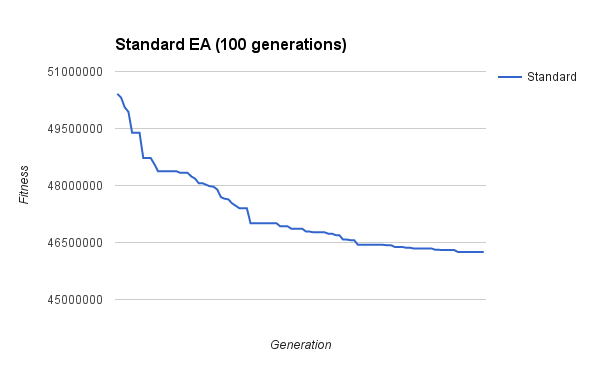
\includegraphics[width=14cm]{img/standard-ea}
	\caption{Resultados obtenidos con el algoritmo genético estándar durante 100 generaciones}
	\label{fig:standard-ea}
\end{figure}

\subsection{Variante \textit{baldwiniana}}

Para mejorar los resultados teníamos que aplicar una técnica de optimización local para explotar un espacio de exploración. Para ello se han utilizado dos técnicas: la \textit{baldwiniana} y la \textit{lamarckiana}.
\\ \\
La \textit{baldwiniana} consiste en optimizar cada uno de los individuos, pero sin usar estos individuos optimizados para generar la nueva población.

\label{sec:opt-local}
\subsubsection{Optimización local}

La técnica de optimización local utilizada es una técnica \textit{2-opt}. En la que se va comprobando como un intercambio de genes en un individuo puede mejorar su coste asociado. El pseudo-código de esta para cada individuo es:

\begin{lstlisting}
do {
	best = S
	for (i = 0 -> solution.length) {
		for (j = i + 1 -> solution.length) {
			T = S
			T[i] = S[j]
			T[j] = S[i]
			T.adjustFitness()
			if (T.fitness < S.fitness) {
				S = T
			}
		}
	}
} while (S.fitness < best.fitness)
\end{lstlisting}

La función \texttt{adjustFitness} es la que calcula el nuevo coste de la solución con la permutación realizada. En un principio usé la misma función de calcular el coste del individuo completo pero ralentizaba tanto el tiempo de cómputo que tuve que buscar una alternativa.
\\ \\
Como al permutar \textit{i} y \textit{j} solo se ven afectadas dos filas y dos columnas de la matriz (el 0.78\% del total de las celdas), calcular el coste del individuo completo era una tontería.
\\ \\
Se cambió esta función para que restase el coste de la solución antigua y se sumen las de la nueva. En pseudo-código:

\begin{lstlisting}
for (k = 0 -> Problem.size) {
	fitness -= w[i][k] * d(oldSol[i][k])
	fitness += w[i][k] * d(newSol[i][k])
	fitness -= w[j][k] * d(oldSol[j][k])
	fitness += w[j][k] * d(newSol[j][k])
	if (k != i && k != j) {
		fitness -= w[k][i] * d(oldSol[k][i])
		fitness += w[k][i] * d(newSol[k][i])
		fitness -= w[k][j] * d(oldSol[k][j])
		fitness += w[k][j] * d(newSol[k][j])
	}
}
\end{lstlisting}

\subsubsection{Primeros resultados}

Usando los mismos parámetros que los definidos en la sección \ref{sec:standard-parameters} se ha llegado a obtener un individuo con coste 44.847.954 (Figura \ref{fig:baldwinian-ea}) que mejoraba en aproximadamente 1.400.000 el resultado obtenido con el algoritmo genético estándar para el conjunto de datos de prueba \texttt{tai256c}. 

\begin{figure}[H]
	\centering
	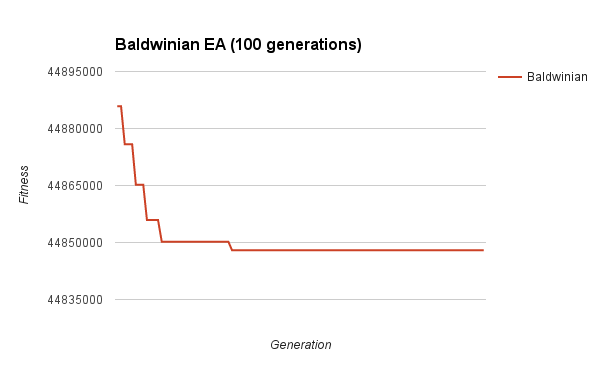
\includegraphics[width=14cm]{img/baldwinian-ea}
	\caption{Resultados obtenidos con la variante \textit{baldwiniana} durante 100 generaciones}
	\label{fig:baldwinian-ea}
\end{figure}

Se puede observar como la solución se queda estancada muy pronto en un óptimo local llegando a alcanzarlo antes de la generación 50.

\subsection{Variante \textit{lamarckiana}}

Usando el mismo método que el descrito en la sección \ref{sec:opt-local} se ha creado la variante \textit{lamarckiana} que se diferencia de la \textit{baldwiniana} en que el individuo optimizado se utiliza para la generación de la nueva población.

\subsubsection{Primeros resultados}

Usando los mismos parámetros que los definidos en la sección \ref{sec:standard-parameters} se ha llegado a obtener un individuo con coste 44.812.496 (Figura \ref{fig:lamarckian-ea}) que mejoraba en aproximadamente 1.400.000 el resultado obtenido con el algoritmo genético estándar y en 35.000 al obtenido con la variante \textit{baldwiniana} en el conjunto de datos de prueba \texttt{tai256c}.

\begin{figure}[H]
	\centering
	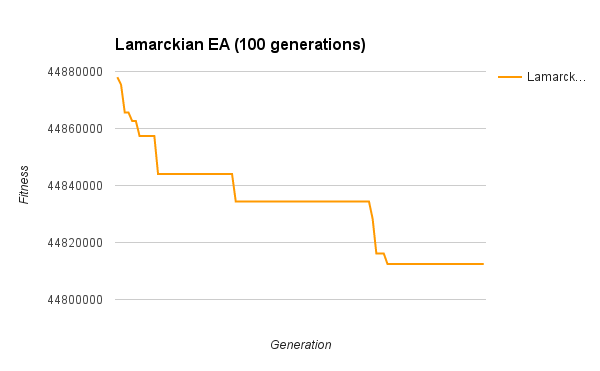
\includegraphics[width=14cm]{img/lamarckian-ea}
	\caption{Resultados obtenidos con la variante \textit{lamarckiana} durante 100 generaciones}
	\label{fig:lamarckian-ea}
\end{figure}

Con esta variante se estanca en un óptimo local más tarde que con la anterior.

\section{Resultados}

\label{sec:comparacion-metodos}
\subsection{Comparación de métodos}

Una vez implementados todos los métodos es el momento de intentar encontrar la mejor solución posible en el conjunto de datos \texttt{tai256c}, para ello, lo primero que hay que decidir es en qué método centrarse.
\\
\\
Se puede observar con claridad que el algoritmo genético estándar, pese a ser muy rápido debe ser descartado (Figura \ref{fig:comparing-standard-with-opt}) pues depende mucho de la población inicial y debemos intentar depender lo menos posible del azar.

\begin{figure}[H]
	\centering
	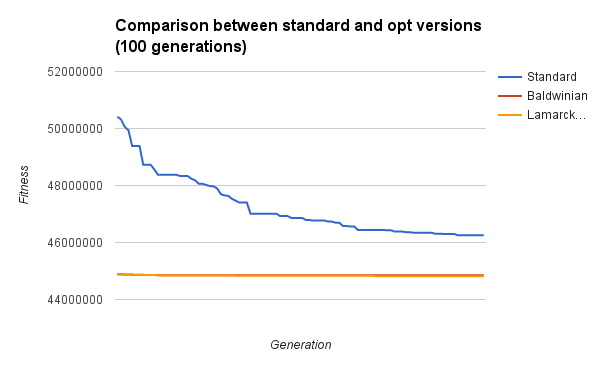
\includegraphics[width=14cm]{img/comparing-standard-with-opt}
	\caption{Resultados obtenidos con todas las variantes implementadas tras 100 generaciones}
	\label{fig:comparing-standard-with-opt}
\end{figure}

La diferencia de los algoritmos con optimización local a la escala de su comparación con el genético estándar es muy chica, por lo que realizamos un \textit{zoom} para compararlos (Figura \ref{fig:comparing-opt}).
\\ \\
La diferencia es considerable y podemos observar como la variante \textit{lamarckiana} funciona bastante mejor que la variante \textit{baldwiniana}.
\\ \\
Por esta razón nos dedicaremos a optimizar los parámetros para mejorar el resultado obtenido con esta variante para acercarnos lo máximo posible a la solución más óptima descubierta hasta ahora (44.759.294).

\begin{figure}[H]
	\centering
	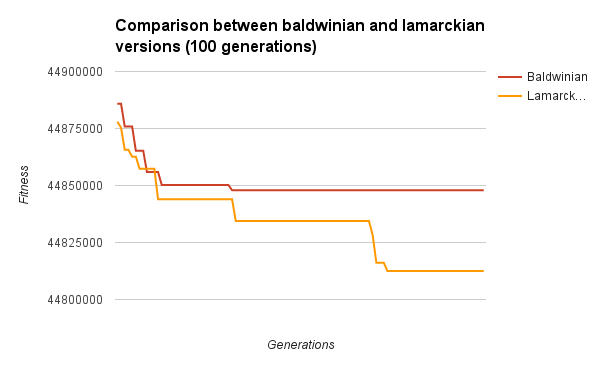
\includegraphics[width=14cm]{img/comparing-opt}
	\caption{Resultados obtenidos con las variantes con optimización local tras 100 generaciones}
	\label{fig:comparing-opt}
\end{figure}

\subsection{Ajuste de parámetros}

En la gráfica presentada en la sección \ref{sec:comparacion-metodos} se puede observar como la variante \textit{lamarckiana} no llega a estancarse del todo tras 100 generaciones, por lo que se aumentaron el número de generaciones a 200 con el objetivo de comprobar si era una impresión acertada. Pero tras varias ejecuciones se vio que no solía mejorarse tras las 100 generaciones. Solo en 1 de 5 ejecuciones, por lo que se mantuvo el número de generaciones.
\\ \\
Para intentar conseguir una mayor variedad de individuos se cambió la probabilidad de mutación aumentando de 0,3 a 0,8 la probabilidad de que mute un individuo y de 0,002 a 0,01 la de un gen. Los resultados obtenidos tampoco diferían demasiado por lo que se probó con valores intermedios entre ambos ya que me parecían muy bajas las probabilidades iniciales dejando finalmente la probabilidad de que un individuo mute a 0,5 y de un gen a 0,005 y se ejecutó varias ocasiones obteniendo unos resultados ligeramente mejores que los que se obtuvieron previamente.

\subsection{Resultado final}

El mejor resultado finalmente se obtuvo con los siguientes parámetros:

\begin{itemize}
	\item Tamaño de población: 100
	\item Número de generaciones: 100 (obtenidos mejor resultado en la 85)
	\item Número de individuos en el torneo: 5
	\item Probabilidad de mutación de individuo: 0,3
	\item Probabilidad de mutación de gen: 0,5
\end{itemize}

El resultado fue 44.790.360 a tan solo 31.066 del mejor resultado obtenido hasta ahora con un algoritmo genético.
\\ \\
La ejecución del algoritmo hasta que encontró este resultado duró 38 minutos y 39 segundos.

\section{Conclusiones}

Lala


%----------------------------------------------------------------------------------------
%	REFERENCIAS
%----------------------------------------------------------------------------------------

\newpage

\bibliography{referencias} %archivo referencias.bib que contiene las entradas 
\bibliographystyle{plain} % hay varias formas de citar

\end{document}